\section{Post hoc omnibus reanalysis of Study 1}
\label{app:pilot}
Fitting model~\eqref{eq:h1} to the 60 Study~1 P1 and P2 runs (six architectures, five seeds)
gives a P1--P2 difference of \PilotEst~pp (SE \PilotSE, Satterthwaite $p=\PilotP$,
$\mathrm{df}=\PilotDf$). This analysis was specified after the Study~1 data were seen; it
motivated Study~2 and supplied its pilot variance components, and it is not confirmatory.

\section{Power analysis}
\label{app:power}
\begin{figure}[h]
\centering
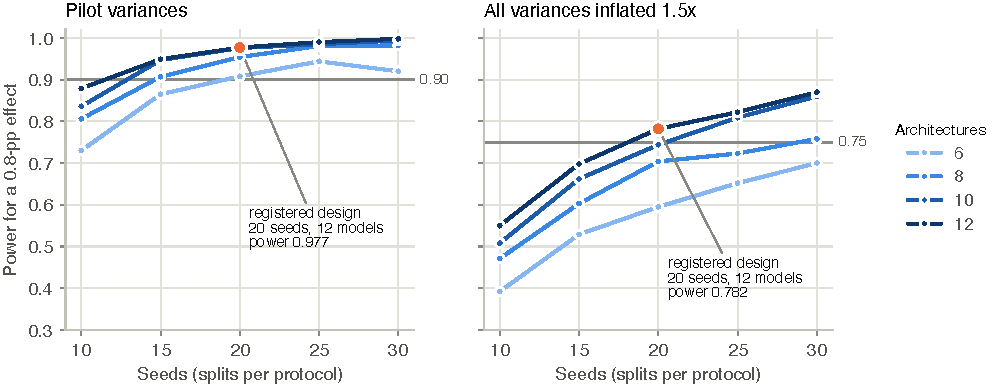
\includegraphics[width=\linewidth]{figures/power.pdf}
\caption{Simulated power of model~\eqref{eq:h1} for a 0.8-pp effect (1,000 simulations per design).
The registered design (twenty seeds, twelve architectures) reaches \PowerChosen{} with pilot
variances and \PowerInflated{} with every variance inflated by half.}
\label{fig:power}
\end{figure}
